\section{El Concepte de 3BLD}

Per començar cal entendre el funcionament d'una resolució de blind, primer el cub és barrejat per una persona i el posa dins d'una capsa o un cube cover\footnote{Un cube cover és una tapa per cubs feta de cartró i que s'utlitza a les competicions}, després es col·loca a la taula boca avall i la persona que l'ha de resoldre es pren el seu temps per respirar. 
Un cop fet això la persona que resol el cub encén el timer i destapa el cub, de manera que el temps comença a comptar i es comença a memoritzar. Un cop acabada la memorització el que resol el cub es tapa els ulls amb un antifaç i comença a resoldre el cub, mentre que una persona externa li posa una cartiluna entre el cub i la seva cara per evitar trampes i mirar per sota de l'antifaç.
Tots aquests passos s'han d'executar perfectament perr asegurar-se de la resolució compti.

\begin{figure}[ht]
    \centering
    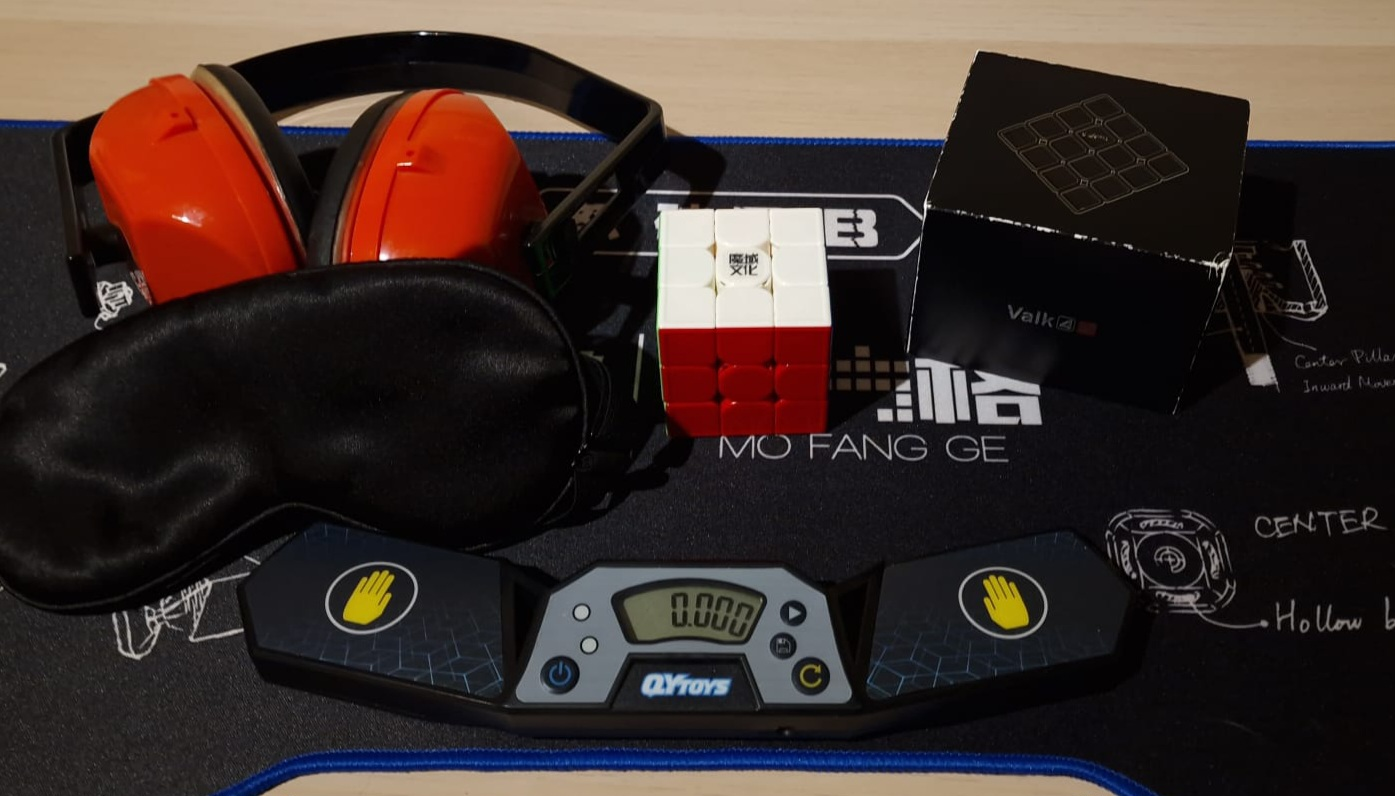
\includegraphics[width=12cm]{img/figures/materials-bld.jpg}
\caption{Materials necessaris per poder executar blind}
    \label{fig:materials-bld}
\end{figure}

En la imatge \ref{fig:materials-bld} es poden veure el timer\footnote{El timer és el compatdor amb la forma de les mans que es veu al centre de la imatge}, l'antifaç, la caixa per cobrir el cub, que en aquest cas jo utlizo una que tinc d'un cub, i a més a més uns cascos d'obra per aïllarte del soroll ambient.

\vspace{0.5cm}
\subsection{Fases de la Resolució}

Com ja he esmentat a la seccio anterior, completar el cub de Rubik amb els ulls tancats, es divideix en dos grans fases, memorització i execució. I dins d'aquestes fases hi han diferents procediments per poder aconseguir fer-ho correctament.

\subsection{Memorització}

Durant aquesta fase de memorització, com ja ho diu el seu nom, s'ha de memoritzar el cub. Molta gent pensa que els speedcubers que practiquem blind memoritzem el cub color per color mitjançant la memòria fotogràfica, però la veritat no és així, perquè la memòria fotogràfica només la té molt poca gent, i bé, jo m'enrecordo dels objectes que tinc a la taula si tanco els ulls ara mateix, però memoritzar el cub d'aquesta manera porta molt de temps i no és la més eficient de fer-ho.
El que fem es convertir aquestes posicions on estan les peçes del cub, que "només" són 20 en lletres i ho fem d'una manera distribuida en ordre que nosaltres ens memoritzem. L'esquema de lletres\footnote{És la distribució de lletres} que utilizo es veu a la figura \ref{fig:letter-scheme}.

\begin{figure}[ht]
    \centering
    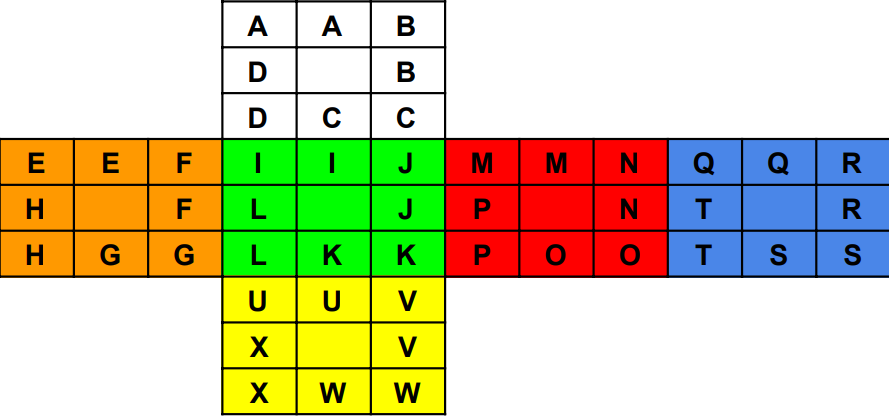
\includegraphics[width=12cm]{img/figures/letter-scheme.png}
\caption{Esquema de Lletres}
    \label{fig:letter-scheme}
\end{figure}

Com es pot veure hi han lletres repetides i això és degut a que hi ha memorització per arestes i memorització per cantonades. Com està mencionat a la secció 1.2.2 en el cub hi ha 8 arestes i 12 cantonades, per tant haig de memoritzar respectivament 12 lletres d'arestes i 8 lletres de cantonades.
Un altre cop tenim el problema de que no és gaire eficient memoritar les lletres una per una i és per això que la manera correcta de fer-ho és la següent. Memoritzar dues lletres i amb aquestes dos lletres formar una paraula de la qual et sigui fàcil pensar en una imatge la qual et pots enrecordar fàcilment. En resum, és convertir parells de lletres en en imatges, per tant ara tenim la meitat d'ítems a memoritzar. Un exemple d'aquesta fusió de lletres és: 
\vspace{0.25cm}

$$ \textrm{Haig de memoritzar les lletres R i B    }  \rightarrow \textrm{   RedBull} $$
$$ \textrm{Haig de memoritzar les lletres A i C   }  \rightarrow \textrm{   Aire Acondicionat (AC és el símbol)} $$

\vspace{0.33cm}

De manera pràctica es comença a memortizar desde la peça UK mirant el color de U, de la lletra en la posició U que és la inicial i treus una lletra i llavors mires a la posciió on ha d'anar aquesta primera lletra que has trobat i mires quina lletra treus, i així fins que memoritzis totes les arestes i després fas el mateix amb les cantonades. És una concepte díficl d'explicar amb paraules i es veu millor al següent exemple. Cal destacar que al començar a memortizar la posició UK la saps perquè col·loques el centre verd mirant cap a tu i el centre blanc mirant cap a dalt.
\\\\BARREJA: F2 B R2 U'L2 U2 B' L' F2 U' B2 U L2 U R2 F2 L2 U' L2 F

\begin{figure}[h!]
    \centering\RubikCubeSolvedWY
    \RubikRotation{Y,F2,B,R2,Up,L2,U2,Bp,Lp,F2,Up,B2,U,L2,U,R2,F2,L2,Up,L2,F}
    \ShowCube{8cm}{0.6}{\DrawRubikCubeF}
    \caption{Cub barrejat per exemple de Blind}
    \label{exemple-memo}
    \end{figure}

Començem mirant all lloc de U K com a l'esquema de lletres i veiem que és blanca a lloc U i taronja al lloc K, llavors ens fixem en l'esquema de lletres en l'aresta blanca-taronja i veiem que és la lletra D. 
Després ens fixem en el lloc de la lletra D i està una peça blanca-verda que és la lletra C, però és un cas especial, que més tard parlo a la secció d'execució però aquesta C es converteix en W, no s'ha de saber res més, només és per tenir el concepte entès. Això ho fem succesivament i obtenim que les lletres totals que ens hem de memoritzar són:

$$ \textrm{Memorització Arestes: DW LA BV PX RI GT N } $$ $$ \textrm{(En aquest cas surten 13 perquè ha sigut una barreja amb cas especial)} $$
$$ \textrm{Memorització Cantonades: U MH VS MC} $$ $$ \textrm{(Igual que amb les arestes al ser un cas especial el valor es veu afectat)} $$
\vspace{0.17cm}
$$ \textrm{Memorització Total DW LA BV PX RI GT NU MH VS MC } $$

\begin{table}[h]
    \begin{minipage}{.5\linewidth}
        \centering
        \begin{tabular}{|c|c|}
            \hline
            Lletres & Transcripció\\
            \hline
            DW & DeU (pronunciació)\\
            \hline
            LA & Los Ángeles\\
            \hline
            BV & BBVA\\
            \hline
            PX & PeiX\\
            \hline
            DF &  DoFí\\
            \hline 
            Ri & RIu  \\
            \hline
        \end{tabular}
    \end{minipage}
    \begin{minipage}{.5\linewidth}
        \centering
        \begin{tabular}{|c|c|}
            \hline
            Lletres & Transcripció\\
            \hline
            GT & Gran Turismo \\
            \hline
            NU & NUt (Femella en anglés)\\
            \hline
            MH & MoHa\\
            \hline
            VS &  VerSuS\\
            \hline 
            MC &  MigCampista\\
            \hline
        \end{tabular}
    \end{minipage} 
\end{table}





\subsection{Execució}

L'execució és la segona fase per completar el cub a cegues i es fa d'una maner molt diferent a la que es fa el cub de manera convencional. Quan resols el cub mirant fas rotacions al cub per buscar les peces i fer moviments, en canvi a les resolucions a cegues el cub no es rota en tota l'execució. Llavors les peces s'aconsegueixen col·locar a lloc gràcies a algoritmes\footnote{És una seqüència de moviments que permet realitzar una tasca}.
\\Com que el cub no ha de rotar, les peces també s'han de quedar en el mateix lloc a l'acabar l'algoritme, és a dir, és executar un algoritme, mous les dues peces que vols i acabes amb la resta del cub igual però amb les dues peces canviades. 
\\\\Hi han diferents nivells d'eficiència d'algoritmes, i es perquè amb els algoritmes més complicats es pot fer de manera més eficient i per tant hi ha menys moviments, però en canvi és més difícl d'aprendre-se'ls. L'explicació darrere d'això és:

$$ \textrm{Quan fas un algoritme fas} \rightarrow Y X Y' X' $$

El que es fa, és executar uns moviments que li direm seqüència Y , que normalment aquesta és per preparar el lloc on les peces es canviaran, després fem una seqüència X, en aquesta el que fem es intercanviar les peces entre elles, després fem la secuencia Y' que és la secuencia y al revés, aquesta el que fa és tornar enrere el moviment fet anteriorment i preparar el retorn de la secuència Y'. FInalment amb la secuencia Y' el que fem retornar el cub a l'estat anterior però amb les peces objectius canviades.
\\\\Un exemple d'això és un intercanvi de tres cantonades, que visualment pas a pas aplicant una seqüència darrera de l'altra es veu:

\begin{figure}[htbp]
    \centering
    \begin{subfigure}
        \centering\RubikCubeSolvedWY
        \RubikRotation{Y,U}
        \ShowCube{7cm}{0.5}{\DrawRubikCubeRU}
    \end{subfigure}
    \begin{subfigure}
        \centering\RubikCubeSolvedWY
        \RubikRotation{Y,U,Rp,D,R}
        \ShowCube{7cm}{0.5}{\DrawRubikCubeRU}
    \end{subfigure}
    \caption{Secuencia Y (Esquerra) i Y X (Dreta)}
\end{figure}

\begin{figure}[htbp]
    \centering
    \begin{subfigure}
        \centering\RubikCubeSolvedWY
        \RubikRotation{Y,U,Rp,D,R,Up}
        \ShowCube{7cm}{0.5}{\DrawRubikCubeRU}
    \end{subfigure}
    \begin{subfigure}
        \centering\RubikCubeSolvedWY
        \RubikRotation{Y,U,Rp,D,R,Up,Rp,Dp,R}
        \ShowCube{7cm}{0.5}{\DrawRubikCubeRU}
    \end{subfigure}
    \caption{Secuencia Y X Y' (Esquerra) i Y X Y'X' (Dreta)}
\end{figure}

Com es pot veure tot acaba per intercanviar 3 cantonades deixant el cub exactament igual, les seqüències són els moviments següents.
\begin{itemize}
    \item X = U
    \item Y = R' D R
    \item X' = U'
    \item Y' = R' D' R
\end{itemize}

Aquesta explicació s'atribueix al mètode més avançat, que no és el que jo utilitzo, ja que el mètode més avançat són 400 algoritmes per cantonades i gairebé 400 per arestes, a més a més es tarden anys d'experiència no només per memoritzar sinó per obtenir la memòria muscular\footnote{És la memòria que fa que nosaltres movem els músculs d'una manera quan pensem una cosa, com quan escrius a l'ordinador.}.

Jo utilitzo el mètode de dificultat mijta-alta però que també té gran eficiència, tinc un mètode per arestes i un mètode per cantonades.

\subsection{El mètode d'execució per les arestes.}

Per les arestes utlitzo el mètode M2, que com ja ho diu el seu nom es basa en el moviment M2, que és el moviment de la capa del mig del cub 2 vegades.

\begin{figure}[h]
    \centering\RubikCubeSolvedWY
    \RubikRotation{Y,M2}
    \ShowCube{7cm}{0.7}{\DrawRubikCubeLU}
    \caption{Exemple de Moviment M2}
\end{figure}
    
Aquest mètode intercanvia les peces d'una manera peculiar, ja que ha de fer dues vegades M2 per tornar a l'estat original i canviar dues peces. Per exemple, fas primer la seqüència Y que col·loca la peça al lloc d'intercanvi, després fas la seqüència X que en aquesta cas és M2 i després fas Y' per retornar la peça intercanviada. Un cop fet això s'han canviat dues peces però el cub no queda igual que abans perquè hem de tornar a fer un intercanvi, aquest segon intercanvi ha de ser amb una seqüència Z X Z' perquè hem d'intercanviar una peça que no sigui la mateixa.
El mètode té aquests casos següents:

\begin{table}[h]
    \begin{minipage}{.5\linewidth}
        \centering
        \begin{tabular}{|c|c|}
            \hline
            A & M2 \\
            \hline
            B & R' U R U' M2 U R' U' R \\
            \hline
            C & U2 M' U2 M' \\
            \hline
            D & L U' L' U M2 U' L U L'  \\
            \hline
            E & B L' B' M2 B L B'  \\
            \hline
            F & B L2 B' M2 B L2 B' \\
            \hline
            G & B L B' M2 B L' B' \\
            \hline
            H & L B L' B' M2 B L B' L' \\
            \hline
            I & D M' U R2 U' M U R2 U' D' M2 \\
            \hline
            J & U R U' M2 U R' U' \\
            \hline
            K & Posició d'intercanvi \\
            \hline
            L & U' L' U M2 U' L U \\
            \hline 
        \end{tabular}
    \end{minipage}
    \begin{minipage}{.5\linewidth}
        \centering
        \begin{tabular}{|c|c|}
            \hline
             M & B' R B M2 B' R' B \\
             \hline
             N & R' B' R B M2 B' R' B R  \\
             \hline
             O & B' R' B M2 B' R B \\
             \hline
             P & B' R2 B M2 B' R2 B \\
             \hline
             Q & U B' R U' B (M2) B' U R' B U' \\
             \hline
             R & U' L U M2 U' L' U \\
             \hline
             S & M2' D U R2 U' M' U R2 U' M D' \\
             \hline
             T & U R' U' M2 U R U'  \\
             \hline
             U & Posició d'intercanvi \\
             \hline
             V & U R2 U' M2 U R2 U' \\
             \hline
             W & M U2 M U2  \\
             \hline
             X & U' L2 U M2 U' L2 U \\
             \hline 
        \end{tabular}
    \end{minipage} 
\end{table}

Exemple d'intercanvi d'arestes L i V:

\begin{figure}[htbp]
    \centering
    \begin{subfigure}
        \centering\RubikCubeSolvedWY
        \RubikRotation{Y,Up,Lp,U}
        \ShowCube{7cm}{0.5}{\DrawRubikCubeRU}
    \end{subfigure}
    \begin{subfigure}
        \centering\RubikCubeSolvedWY
        \RubikRotation{Y,Up,Lp,U,M2}
        \ShowCube{7cm}{0.5}{\DrawRubikCubeRU}
    \end{subfigure}
    \caption{Secuencia Y (Esquerra) i Y X (Dreta)}
\end{figure}

\begin{figure}[htbp]
    \centering
    \begin{subfigure}
        \centering\RubikCubeSolvedWY
        \RubikRotation{Y,Up,Lp,U,M2,Up,L,U}
        \ShowCube{7cm}{0.5}{\DrawRubikCubeRU}
    \end{subfigure}
    \begin{subfigure}
        \centering\RubikCubeSolvedWY
        \RubikRotation{Y,Up,Lp,U,M2,Up,L,U,U,R2,Up}
        \ShowCube{7cm}{0.5}{\DrawRubikCubeRU}
    \end{subfigure}
    \caption{Secuencia Y X Y' (Esquerra) i Y X Y'Z (Dreta)}
\end{figure}

\begin{figure}[h!]
    \centering
    \begin{subfigure}
        \centering\RubikCubeSolvedWY
        \RubikRotation{Y,Up,Lp,U,M2,Up,L,U,U,R2,Up,M2}
        \ShowCube{7cm}{0.5}{\DrawRubikCubeRU}
    \end{subfigure}
    \begin{subfigure}
        \centering\RubikCubeSolvedWY
        \RubikRotation{Y,Up,Lp,U,M2,Up,L,U,U,R2,Up,M2,U,R2,Up}
        \ShowCube{7cm}{0.5}{\DrawRubikCubeRU}
    \end{subfigure}
    \caption{Secuencia Y X Y'Z'X (Esquerra) i Y X Y'Z X Z' (Dreta)}
\end{figure}

Llavors així és com es canviarien dues arestes amb el mètode M2, en aquest cas L i V.

\subsection{Mètode d'execució per les Cantonades}

Per les cantonades utlitzo el mètode orozco, que utlitza un sistema similar al M2, ja que fa les seqüències Y X Y'X' i Z A Z' A' però en aquest cas la seqüència Z és diferent perquè es troba al segon lloc. De manera simple, si a la memorització tens la lletra en segon lloc has de fer l'algoritme alternatiu.
Els casos d'orozco són els següents:

\begin{table}[h]
    \begin{minipage}{.5\linewidth}
        \centering
        \begin{tabular}{|c|c|} 
            \hline
            \textbf{AB} & Basic A Perm \\
            \hline
            \textbf{DB} & U' (A Perm) U \\
            \hline
            \textbf{EB} & [R: [R D R', U]] \\
            \hline
            \textbf{FB} & [R': [U', R' D' R]] \\
            \hline
            \textbf{GB} & [U, R' D R] \\
            \hline
            \textbf{HB} & [R D' R', U'] \\
            \hline
            \textbf{IB} & [R: [R D R', U2]] \\
            \hline
            \textbf{KB} & [D': [U, R' D R]] \\
            \hline
            \textbf{LB} & [D: [U, R' D' R]] \\
            \hline
            \textbf{OB} & [R D R', U'] \\
            \hline
            \textbf{PB} & [U, R' D' R] \\
            \hline
            \textbf{RB} & [R': [U2, R' D' R]] \\
            \hline
            \textbf{SB} & [U, R' D2 R] \\
            \hline
            \textbf{TB} & [D: [R D' R', U']] \\
            \hline
            \textbf{UB} & [x': [R U R', D2]] \\
            \hline
            \textbf{VB} & [D' x': [R U R', D2]] \\
            \hline
            \textbf{WB} & [D x: [D2, R' U' R]] \\
            \hline
            \textbf{XB} & [x: [D2, R' U' R]] \\
            \hline 
        \end{tabular}
    \end{minipage}
    \begin{minipage}{.5\linewidth}
        \centering
        \begin{tabular}{|c|c|}
            \hline
            \textbf{BA} & Reverse A Perm \\
            \hline
            \textbf{BD} & U' (Reverse A Perm) U \\
            \hline
            \textbf{BE} & [R: [U, R D R']] \\
            \hline
            \textbf{BF} & [R': [R' D' R, U']] \\
            \hline
            \textbf{BG} & [R' D R, U] \\
            \hline
            \textbf{BH} & [U', R D' R'] \\
            \hline
            \textbf{BI} & [R: [U2, R D R']] \\
            \hline
            \textbf{BK} & [D': [R' D R, U]] \\
            \hline
            \textbf{BL} & [D: [R' D' R, U]] \\
            \hline
            \textbf{BO} & [U', R D R'] \\
            \hline
            \textbf{BP} & [R' D' R, U] \\
            \hline
            \textbf{BR} & [R': [R' D' R, U2]] \\
            \hline
            \textbf{BS} & [R' D2 R, U] \\
            \hline
            \textbf{BT} & [D: [U', R D' R']] \\
            \hline
            \textbf{BU} & [x': [D2, R U R']] \\
            \hline
            \textbf{BV} & [D' x': [D2, R U R']] \\
            \hline
            \textbf{BW} & [D x: [R' U' R, D2]] \\
            \hline
            \textbf{BX} & [x: [R' U' R, D2]] \\
            \hline 
        \end{tabular}
    \end{minipage} 
    \caption{Algorimtes orozco}
\end{table}

A la columna de l'esquerra hi ha els corresponents a la primera lletra del parell i a la dreta els corresponents a la segona lletra del parell. \textit{A perm} és un cas del cub de rubik normal que es fa (R' U' R' D' R U' R' D R U R' D' R U R' D R2).

\begin{table}[h]
    \begin{minipage}{.5\linewidth}
        \centering
        \begin{tabular}{|c|c|}
            \hline
            \textbf{NB} & [U, R' D R D' R' D' R] \\
            \hline
            \textbf{QB} & [R' D R D' R' D' R, U] \\
            \hline
        \end{tabular}
    \end{minipage}
    \begin{minipage}{.5\linewidth}
        \centering
        \begin{tabular}{|c|c|}
            \hline
            \textbf{BN} & [R' D R D' R' D' R, U] \\
            \hline
            \textbf{BQ} & [U, R' D R D' R' D' R] \\
            \hline 
        \end{tabular}
    \end{minipage} 
    \caption{Excepcions del mètode}
\end{table}



Aquests algoritmes estan escrits en una notació\footnote{Manera d'escriure els algoritmes} diferenti [Y,X]. El fet que estigui entre claudators indica que s'ha de fer en l'ordre Y X Y' X'. És una mica més díficil de visualitzar però més fàcil a l'hora d'aplicar aquest mètode.
Exepmle d'intercanvi de dues cantonades P i H

\begin{figure}[h!]
    \centering
    \begin{subfigure}
        \centering\RubikCubeSolvedWY
        \RubikRotation{Y,U}
        \ShowCube{7cm}{0.5}{\DrawRubikCubeLU}
    \end{subfigure}
    \begin{subfigure}
        \centering\RubikCubeSolvedWY
        \RubikRotation{Y,U,Rp,Dp,R}
        \ShowCube{7cm}{0.5}{\DrawRubikCubeLU}
    \end{subfigure}
    \caption{Secuencia Y (Esquerra) i Y X (Dreta)}
\end{figure}

\begin{figure}[h!]
    \centering
    \begin{subfigure}
        \centering\RubikCubeSolvedWY
        \RubikRotation{Y,U,Rp,Dp,R,Up}
        \ShowCube{7cm}{0.5}{\DrawRubikCubeLU}
    \end{subfigure}
    \begin{subfigure}
        \centering\RubikCubeSolvedWY
        \RubikRotation{Y,U,Rp,Dp,R,Up,Rp,D,R}
        \ShowCube{7cm}{0.5}{\DrawRubikCubeLU}
    \end{subfigure}
    \caption{Secuencia Y X Y' (Esquerra) i Y X Y' X'(Dreta)}
\end{figure}

\begin{figure}[h!]
    \centering
    \begin{subfigure}
        \centering\RubikCubeSolvedWY
        \RubikRotation{Y,U,Rp,Dp,R,Up,Rp,D,R,Up}
        \ShowCube{7cm}{0.5}{\DrawRubikCubeLU}
    \end{subfigure}
    \begin{subfigure}
        \centering\RubikCubeSolvedWY
        \RubikRotation{Y,U,Rp,Dp,R,Up,Rp,D,R,Up,R,Dp,Rp}
        \ShowCube{7cm}{0.5}{\DrawRubikCubeLU}
    \end{subfigure}
    \caption{Secuencia Y X Y' X' Z (Esquerra) i Y X Y' X' Z A(Dreta)}
\end{figure}

\begin{figure}[h!]
    \centering
    \begin{subfigure}
        \centering\RubikCubeSolvedWY
        \RubikRotation{Y,U,Rp,Dp,R,Up,Rp,D,R,Up,R,Dp,Rp,U}
        \ShowCube{7cm}{0.5}{\DrawRubikCubeLU}
    \end{subfigure}
    \begin{subfigure}
        \centering\RubikCubeSolvedWY
        \RubikRotation{Y,U,Rp,Dp,R,Up,Rp,D,R,Up,R,Dp,Rp,U,R,D,Rp}
        \ShowCube{7cm}{0.5}{\DrawRubikCubeLU}
    \end{subfigure}
    \caption{Secuencia Y X Y' X' Z A Z' (Esquerra) i Y X Y' X' Z A Z' A'(Dreta)}
\end{figure}

Com a orientació [Y,X] i [Z,A] són a la taula d'algoritmes PB i BH.

